\chapter{Évaluation}
\label{eval}

\section{Logiciels de construction}

\subsection{Ant}

\subsection{Maven}

\section{Serveur de l'intégration continue}

\subsection{Definition des critères}

En dessous vous trouvez les critères avec une bref déscription qui seront utilisé pour evaluer les quatres serveurs de l'intégration continue qui ont été choisit pour ce travail. \footnote{\cite{ibmciserver}}

\begin{enumerate}
\item \textbf{Caractéristiques du produit} \\
\textit{Les charactéristiques du produit sont l'aspect le plus important quand on choisit un serveur d'IC. On doit savoir les éxigences qu'une entreprise a et de ce point de vue selectionner un logiciel.}
	\begin{itemize}
		\item Intégration avec des outils de gestion des versions \\
		\textit{Est l'outil que nous utilisons supporté? Quelles outils sont supporté?}
		\item Intégration avec l'outil de construction \\
		\textit{Est notre langage de programmation (compilateur) et notre outil de construction supporté?}
		\item Information en retour \\
		\textit{Quelles méthodes de l'information en retour existe et sont ils suffisant pour nous?}
		\item Labeling \\
		\textit{Est-il possible de donner des identifiers à des versions d'un logiciel?}
		\item Extensibilité \\
		\textit{Est-il possible d'écrire des extension propre pour le serveur si necessaire?}
	\end{itemize}
\item \textbf{Générale}
	\begin{itemize}
		\item Fiabilité et longévité
		\item Environnement cible
		\item Infrastructure
		\item Couts
		\item Type de logiciel
	\end{itemize}
\item \textbf{Taille de la communauté}
	\begin{itemize}
		\item Nombre d'utilisateurs
		\item Nombre de plug-ins
	\end{itemize}
\item \textbf{Utilisation}
	\begin{itemize}
		\item Facilité d'utilisation
		\item Complexité de l'installation
	\end{itemize}
\end{enumerate}
\newpage
\begin{landscape}
\subsection{Apercu des resultats}
\begin{table}[H]
	\centering
		\begin{tabular}{lp{4cm}p{4cm}p{4cm}p{4cm}} \toprule
			\textbf{Critères} & \href{https://jenkins-ci.org}{\textbf{Jenkins}} & \href{https://www.jetbrains.com/teamcity/}{\textbf{TeamCity}} & \href{https://travis-ci.org}{\textbf{Travis CI}} & \href{https://www.visualstudio.com/en-us/products/tfs-overview-vs.aspx}{\textbf{Team Foundation Server}} \\ \midrule
			\rowcolor{GrayRow}\textbf{Caractéristique du produit} &  &  &  &  \\ \midrule[0.16em]
			Outils de gestion des versions & Subversion/CVS(+plugins) & Subversion/CVS(+plugins) & github/Git & Git/TFVC \\ \midrule
			Outils de construction & & & + & \\ \midrule
			Information en retour & & & + & \\ \midrule
			Labeling & & & - & \\ \midrule
			Extensibilité & ++ & + & - & -- \\ \midrule
			\rowcolor{GrayRow}\textbf{Générale} &  &  &  &  \\ \midrule[0.16em]
			Fiabilité et longévité & ++ & ++ & ++ & ++ \\ \midrule
			Environnement cible & tous & tous & Linux & Microsoft Windows \\ \midrule
			Infrastructure & On-premises & On-premises & On-premises/SaaS & On-premises/SaaS \\ \midrule
			Couts & gratuit & Freemium* & Freemium* & Freemium \\ \midrule
			Type de logiciel & Open Source (MIT) & Propriétaire & Open Source (MIT) & Propriétaire \\ \midrule
			\rowcolor{GrayRow}\textbf{Taille de la communauté} & & & & \\ \midrule[0.16em]
			Nombre d'utilisateurs & many & many & medium & many \\ \midrule
			Nombre de plugins & ++ & + & - & - \\ \midrule
			\rowcolor{GrayRow}\textbf{Utilisation} &  &  &  &  \\ \midrule[0.16em]
			Facilité d'utilisation & many & many & facile & many \\ \midrule
			Complexité de l'installation & many & many & facile & many \\
			\bottomrule[0.16em]
		\end{tabular}
	\caption{Serveurs de l'IC}
	\label{tab:serveurs_eval}
\end{table}
Freemium = C'est gratuit pour la version base, mais ca coute pour des editions plus grande (entreprise).\\
* free for open source projects
\footnote{\citep{jenkinsplugins} \citep{teamcityenv} \citep{tfsversioncontrol}}

\end{landscape}
\newpage

\subsection{Jenkins}

\subsection{TeamCity}
\newpage
\subsection{Travis CI}
\begin{wrapfigure}{r}{0.4\textwidth}
  \begin{center}
    
\includegraphics[width=0.38\textwidth]{bilder/Travis-CI-logo}
  \end{center}
  \caption{Travis CI Logo}
\end{wrapfigure}
\paragraph{Characteristique du produit}
Travis CI est un serveur de l'intégration continue très facile à mettre en service et avec une intégration excellente avec \href{https://github.com/}{github.com}. Il supporte beaucoup de différent langage et outil de construction. La liste complète peuvent être trouver dans la documentation\footnote{\citep{traviscidocs}}. Mais il seulement supporte git comme outil de gestion des versions.\\
De plus il offre multiple voies d'information en retour. Le plus facile est par email, mais il y a aussi la possibilité d'envoyer des messages par IRC, Slack, HipChat etc.\footnote{traviscinotification}. Chaque construction recoit un identificateur numerique, mais il n'est pas possible de le changer. Il y a une API pour accéder à Travis (SaaS), mais l'extensibilité semble limité.

\paragraph{Générale}
Il existe trois version de Travis CI.
\begin{itemize}
	\item \href{https://travis-ci.org/}{Travis CI for Open Source}
	\item \href{https://travis-ci.com/}{Travis Pro}
	\item \href{https://enterprise.travis-ci.com/}{Travis Enterprise}
\end{itemize}
Les deux première versions sont accessible comme SaaS. Une version est pour des projets Open Source qui est gratuite et l'autre est pour des projets avec un dépot de github privée qui coute. La troisième version est pour des entreprises qui veulent mettre l'infrastructure comme des serveurs à disposition eux-mêmes.

\paragraph{Taille de la communauté}
Travis CI affirme sur la page web qu'il y a 246506 projets Open Source qui sont testé et intégré sur leur platform. Sur la nombre d'utilisateurs des deux versions commercial il n'y a pas d'information.

\paragraph{Utilisation}
L'utilisation de Travis CI est très pratiques est facile. Si on a déja un dépot sur github, il faut seulement trois pas pour lancer l'intégration continue avec Travis.

\begin{enumerate}
	\item Login avec le compte de github sur travis
	\item Choisir le dépot
	\item Écrire un fichier .travis.yml pour définir la configuration
\end{enumerate}

Après ça chaque fois qu'il y a un changement sur le dépot les testes et la construction seras executé automatiquement. Pour construire notre projet de test en java (maven), d'executer les testes avec trois différent version de java et envoyer un email à une adresse si quelque chose ne marche pas, le fichier en bas suffisait. De plus vous trouver un apercu de l'interface d'administration de travis.

\begin{figure}[H]
	\centering
		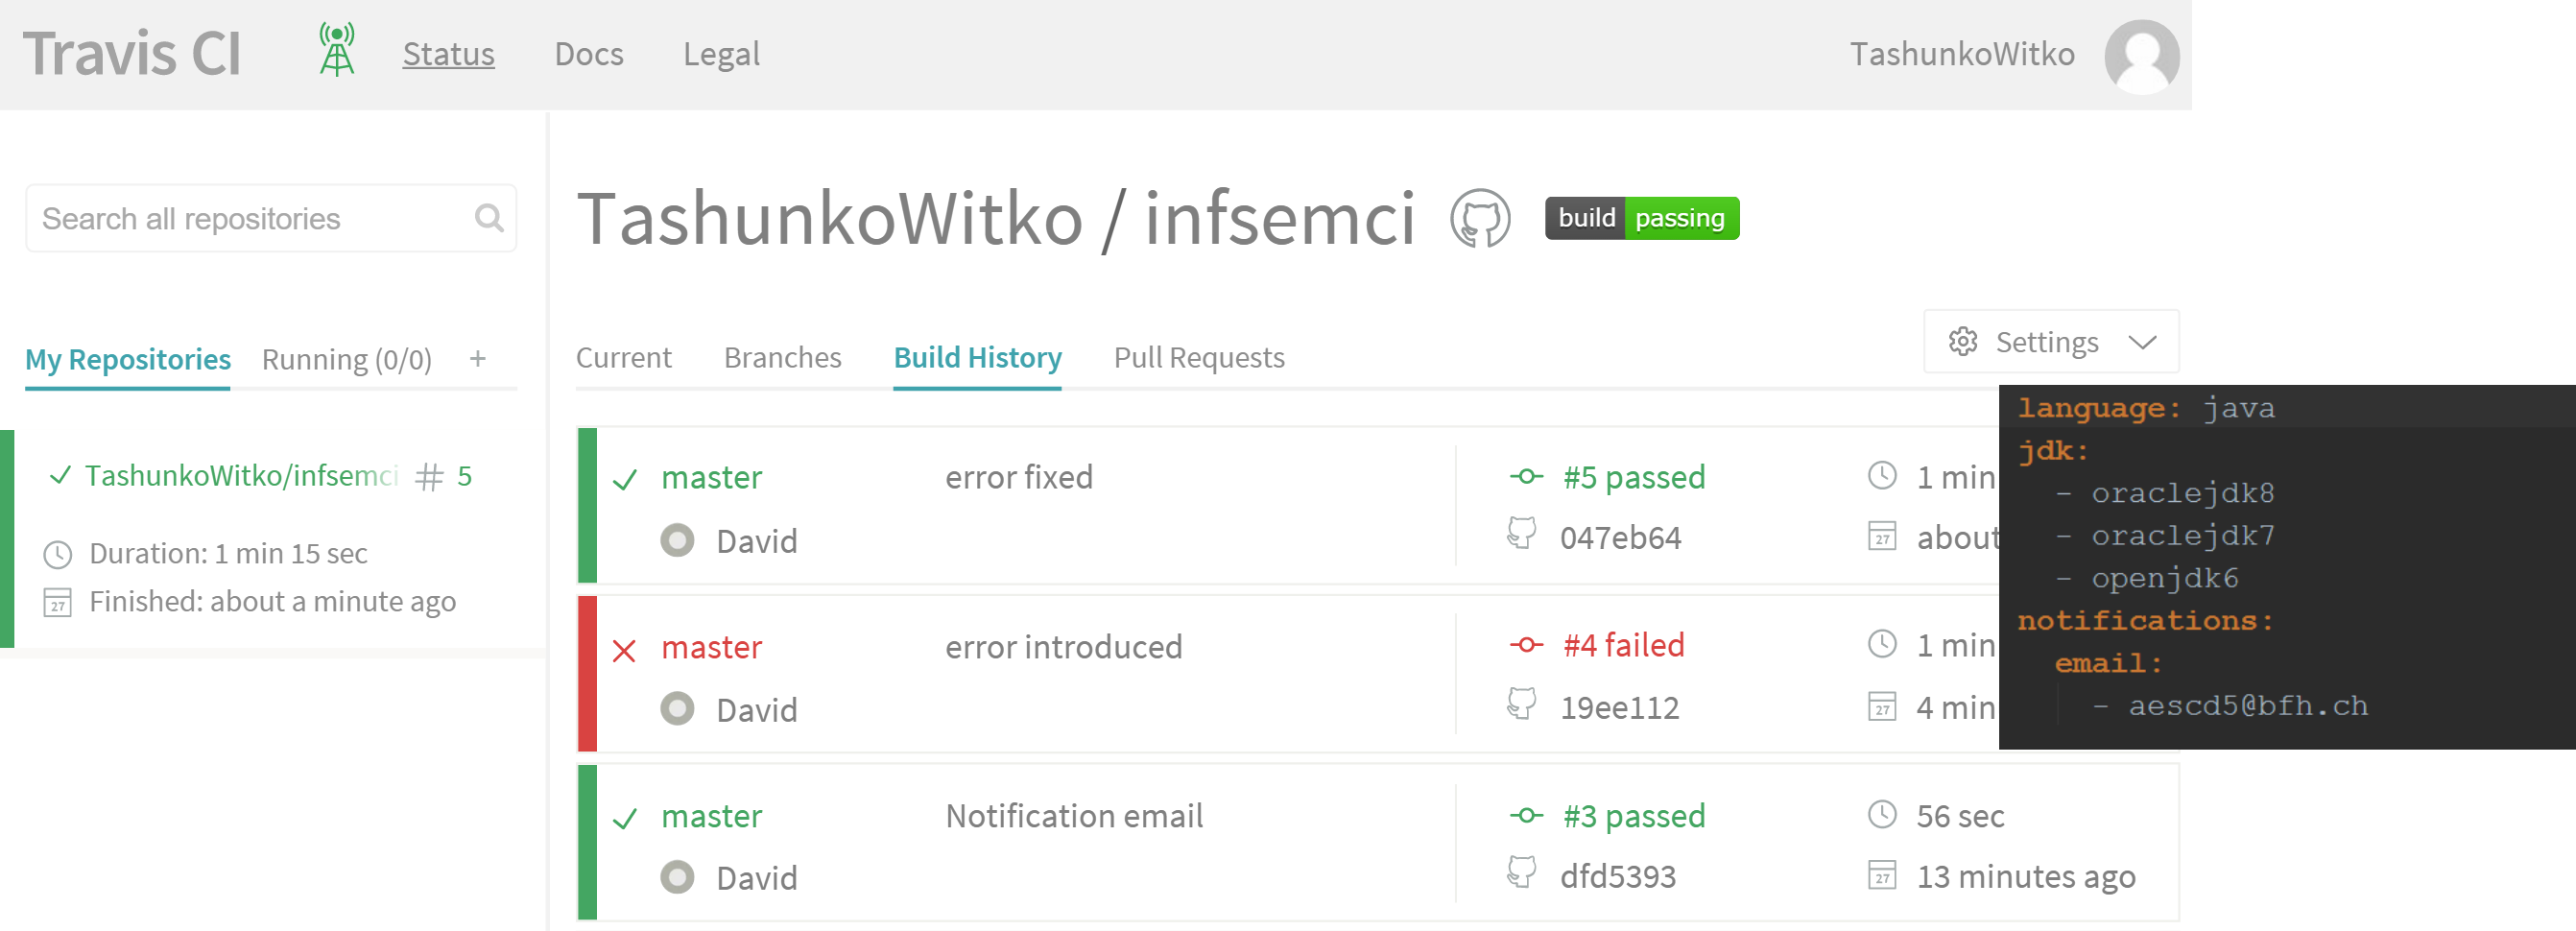
\includegraphics[scale=0.2]{bilder/travisciymlfile}
	\caption{Travis intérface d'administration et yml fichier}
	\label{fig:travisgui}
\end{figure}

\subsection{Team Foundation Server}



